\usetikzlibrary{arrows.meta,calc}
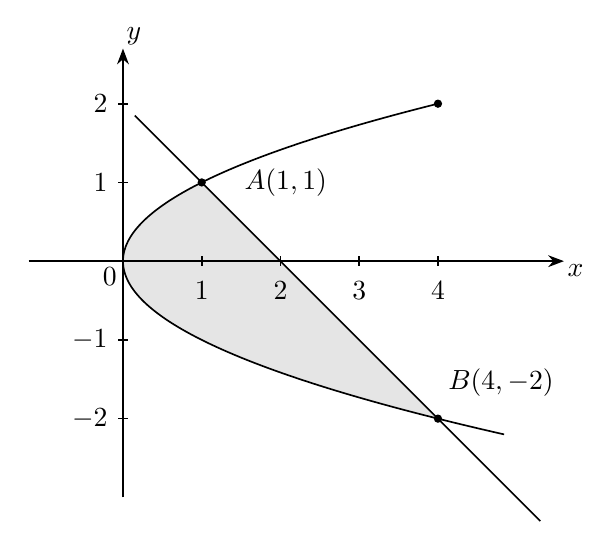
\begin{tikzpicture}[x=1cm,y=1cm,line width=.6pt,font=\normalsize,>=Stealth]
\coordinate (O) at (0,0);
\coordinate (A) at (1,1);
\coordinate (B) at (4,-2);
\coordinate (Uend) at (4,2);
\coordinate (XaxisStart) at (-1.2,0);
\coordinate (XaxisEnd) at (5.6,0);
\coordinate (YaxisStart) at (0,-3.0);
\coordinate (YaxisEnd) at (0,2.7);
\coordinate (LabStart) at (0.15,1.85);
\coordinate (LabEnd) at (5.3,-3.3);
% Shading bounded by x=y^2 and x=2-y, -2<=y<=1.
\fill[gray!20,domain=1:-2,samples=121] plot ({(\x)^2},\x) -- cycle;
% axes
\draw[->] (XaxisStart)--(XaxisEnd) node[below right,inner sep=0pt,xshift=1pt,yshift=-1pt] {$x$};
\draw[->] (YaxisStart)--(YaxisEnd) node[above right,inner sep=0pt,xshift=1pt,yshift=1pt] {$y$};
\foreach \k in {1,2,3,4} {\draw (\k,0.06)--(\k,-0.06); \node[below,inner sep=2pt] at (\k,-0.18) {$\k$};}
\foreach \m in {-2,-1,1,2} {\draw (0.06,\m)--(-0.06,\m); \node[left,inner sep=3pt] at (-0.08,\m) {$\m$};}
\node[below left,inner sep=0pt,xshift=-2pt,yshift=-2pt] at (O) {$0$};
% boundaries and curve
\draw[domain=-2.2:2.0,samples=121] plot ({(\x)^2},\x);
\draw (LabStart)--(LabEnd);
% points
\fill (A) circle (1.5pt);
\fill (B) circle (1.5pt);
\fill (Uend) circle (1.5pt);
% labels
\node[right,inner sep=1pt] at (1.5,1) {$A(1,1)$};
\node[above right,inner sep=2pt] at (4.05,-1.80) {$B(4,-2)$};
\end{tikzpicture}
